\section{Les séquences de codage}
\subsection{Les formats complexes}
\begin{frame}{L'assemblage de types}
  Presque tous les langages de programmation utilisent une notion de
  \emph{types de base} et de \emph{composition de types}.
  \begin{block}{Types de base}
    Les langages ont presque tous un type \emph{entier} et un type
    \emph{flottant} (certains n'ont pas le premier). Il y a aussi souvent un
    type \emph{booléen} et un type \emph{caractère} qui désigne un caractère.

    Ces types de base sont les éléments les plus
  \end{block}
  \begin{block}{Assemblage}
    Les assemblages typiques sont les \textbf{assemblages par répétition}
    (structures de \emph{tableau} (taille fixe), de vecteur ou de liste
    (taille arbitraire), mais aussi des \textbf{assemblages hétérogènes} de
    taille fixe.

    Une dernière option est l'assemblage de type \emph{variante} qui consiste
    à pouvoir mettre dans un même emplacement un type ou un autre. Certains
    langages ne spécialisent même pas les variables.
  \end{block}
\end{frame}
\begin{exercice}
  \begin{exercicelet}{Types simples ou composés}
    \begin{questions}
    \item Identifiez dans les types suivants lesquels sont susceptibles
      d'êtres des types de base et lesquels sont plutôt des types construits
      par assemblage:
      \begin{itemize}
      \item Un nombre entier positif ou nul
      \item Un nombre complexe
      \item Un point dans l'espace
      \item Un nombre avec un très grand nombre de chiffres non fixé à
        l'avance
      \item Un intervalle
      \item Une date
      \item Un étudiant (nom, prénom, date de naissance)
      \item Un caractère
      \item Une chaîne de caractères
      \end{itemize}
    \end{questions}
  \end{exercicelet}
  \begin{exercicelet}{Une date}
    \begin{questions}
    \item Décrivez à partir de quels éléments on peut composer une donnée qui
      représente un moment précis de la journée.
    \item Discutez les éléments précis selon que l'on considère qu'un moment
      est pris à la seconde près ou beaucoup plus précis.
    \end{questions}
  \end{exercicelet}
\end{exercice}
\begin{frame}{Éléments de taille variable}
  \begin{itemize}
  \item[\ddialogquestion] Il arrive que l'on veuille représenter une structure
    complexe qui compte un nombre variable d'autres structures.
  \item[\dialoginformation] Par exemple une chaîne de caractères!
  \item Problème de détection de la fin.
  \item Codage du nombre d'éléments, ou séquence de fin.
  \item[\ddialogwarning] Lors de la construction de structures complexes à
    partir de structures élémentaires, on peut externaliser la structure de
    taille variable.
  \item[\ddialoginformation] Une structure de taille fixe est plus facilement
    manipulable (notamment pour en faire des vecteurs ou des listes).
  \end{itemize}
\end{frame}
\begin{frame}{Représentation en mémoire}
  \begin{block}{Représentation dans un fichier}
    \begin{itemize}
    \item L'unité de base est l'octet
    \item Les données peuvent être indexées (on connaît le début de chaque
      donnée)
    \item Les données peuvent être typées (on connait le type de chaque
      donnée)
    \item Compromis entre taille occupée et résistance aux erreurs ou
      déchiffrabilité
    \end{itemize}
  \end{block}
  \begin{block}{Représentation en mémoire vive}
    \begin{itemize}
    \item Les données simples ont souvent une représentation en mémoire qui
      occupe un nombre d'octets contigus fixe.
    \item Les données composites sont stockées par juxtaposition des données
      élémentaires qui les composent.
    \item Les données de taille variables sont \emph{externalisées}. On les
      connaît alors par leur \textbf{adresse}, l'emplacement mémoire où elles
      sont stockées.
    \end{itemize}
  \end{block}
\end{frame}
\subsection{La représentation en mémoire}
\begin{frame}{Du nombre de bits d'un processeur}
  \begin{itemize}
  \item Un processeur manipule des données avec une taille fixe
  \item[\dialogwarning] Il y a parfois plusieurs tailles manipulables
  \item Historique:
    \begin{itemize}
    \item Ordinateurs 8 bits: 1972--1985
    \item Ordinateurs 16 bits: 1975--1990
    \item Ordinateurs 32 bits: 1986--maintenant
    \item Ordinateurs 64 bits: 1992/2003--maintenant
    \end{itemize}
  \item Pour les flottants ou les données graphiques, il y a des circuits
    spécialisés qui ont des tailles différentes (plus grandes)
  \item Les données de taille supérieure doivent être manipulées en plusieurs
    opérations et ne sont pas des données simples
  \item[\dialoginformation] C'est la taille du \emph{mot-machine}.
  \end{itemize}
\end{frame}
\begin{frame}{Données simples du C}
  \begin{itemize}
  \item \texttt{char} (C2 8 bits)
  \item \texttt{short int} (C2 ≥16 bits)
  \item \texttt{int} (C2 ≥16 bits, usuellement 32)
  \item \texttt{long int} (C2 ≥32 bits)
  \item \texttt{long long int} (C2 ≥64 bits)
  \item \texttt{float} est l'IEEE754 simple précision (32 bits),
    \texttt{double} est la double précision (64 bits), \texttt{long double}
    est la précision étendue ou quadruple selon les processeurs, ≥80 bits).
  \item une \emph{adresse} permet de désigner une autre donnée dans la
    mémoire. Leur taille a varié dans l'histoire de l'informatique.
  \item N'oubliez pas qu'un nombre peut cacher un champ de bits
  \item Des versions \texttt{unsigned} de toutes les longueurs d'entiers
    existent et permettent de choisir le codage NAT au lieu de C2.
  \end{itemize}
\end{frame}
\begin{frame}{Les modèles de programmation 32 et 64 bits}
  Besoin de garder la compatibilité des codes sources.

  En C et en C++ les types changent de taille.
  \begin{center}
    \begin{tabular}{l|ccccc|l}
      &Taille&Taille&Taille&Taille&Taille&Exemples\\
      Modèle&\texttt{short}&\texttt{int}&\texttt{long}&adresse&\texttt{long}&de\\
      &\texttt{int}&&&&\texttt{long}&Compilateurs\\\hline
      32 bits&16&32&32&32&---&\\\hline
      LP64&16&32&64&64&---&Tous sauf...\\\hline
      ILP64&16&64&64&64&---&Exceptions...\\\hline
      LLP64&16&32&32&64&64&Microsoft...
    \end{tabular}
  \end{center}
\end{frame}
\begin{frame}{Alignement}
  \begin{block}{Qu'est-ce que l'alignement ?}
    Les processeurs présentent des contraintes techniques pour l'adressage des
    données. Une opération sur une donnée de type simple en mémoire doit se
    faire avec une adresse multiple de sa taille.

    Les types de taille supérieure au mot-machine sont de toute façon
    manipulée en morceaux indépendants.
  \end{block}

  \begin{example}
    Sur une machine 32 bits, un \texttt{int} (4 octets) ne peut pas commencer
    à l'adresse \texttt{0x00000002}. Il commence soit à l'adresse
    \texttt{0x00000000}, soit \texttt{0x00000004}. Par contre, un
    \texttt{short int} de 16 bits pourra commencer à cette adresse.
  \end{example}
\end{frame}
\begin{frame}{L'alignement dans les données composées}
  Sauf exception, l'alignement doit être respecté pour toutes les composantes
  de la donnée composée. L'adresse de la donnée composée est l'adresse de la
  première composante, et chaque composante doit être alignée correctement
  vis-à-vis de sa taille.
\end{frame}
\begin{exercice}
  \begin{exercicelet}{Stockage d'une date (suite)}
    Une date est composée des éléments suivants:
    \begin{itemize}
    \item Une année (disons de -2 milliards à +2 milliards)
    \item Un mois, un jour du mois
    \item Un fuseau horaire qui est une «~adresse~»
    \item Une heure, une minute (entiers)
    \item Un nombre de secondes qui est un flottant simple précision
    \end{itemize}
    \begin{questions}
    \item Dites quels sont les types de base du C à utiliser pour coder cette
      information, d'après les limites connues de stockage pour chaque
      type. Utilisez les tailles les plus petites possibles.
    \item Donnez leur noms à la fois dans un modèle 32 bits et un modèle 64
      bits.
    \item Si on avait voulu aller de -5 milliards à +5 milliards d'années,
      quel type aurait-on dû utiliser ?
    \item Si les données sont dans l'ordre indiqué dans un type composé,
      précisez à quel moment les contraintes d'alignement provoquent des
      «~trous~» dans la structure.
      \begin{xcorrection}
        On commence par 4 octets, puis 2 fois un octet. Puisqu'une adresse
        fait 4 ou 8 octets, il faut là un trou qui fait 2 octets (alignement
        sur 4 octets) ou 6 octets (alignement sur 8 octets).

        Après, on a encore 2 octets (des \texttt{char} suffisent pour heures
        et minutes), suivi d'un \texttt{float} donc sur 4 octets. Encore 2
        octets de trous sont donc nécessaires.
      \end{xcorrection}
    \item Quelle est la taille totale de la structure (avec les trous) ?
      \begin{xcorrection}
        En 32 bits pour une adresse: 4+2+2+4+2+2+4=20 octets.

        En 64 bits pour une adresse: 4+2+6+8+2+2+4=28 octets.

        Si on veut aller jusqu'à 5 milliards, il faut rajouter 4 octets à
        chaque fois.
      \end{xcorrection}
    \end{questions}
  \end{exercicelet}
\end{exercice}
\begin{frame}{Grand et petit-boutien (little/big-endian)}
  \begin{itemize}
  \item Valeur %
    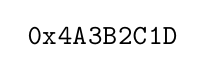
\begin{tikzpicture}[remember picture,%
      every node/.style={font=\ttfamily,anchor=west,inner sep=0pt}]%
      \node (d0) {0x}; \node (d1) at (d0.east) {4A}; \node (d2) at (d1.east)
      {3B}; \node (d3) at (d2.east) {2C}; \node (d4) at (d3.east) {1D};
    \end{tikzpicture}, adresse \texttt{0x00000000} ?
  \item<2->[\dialogquestion] Plusieurs représentations possibles:
    \begin{itemize}
    \item 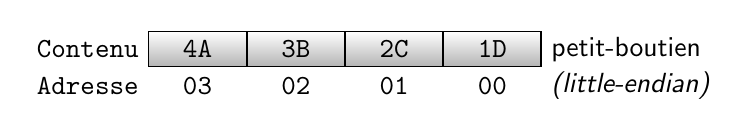
\begin{tikzpicture}[remember picture,%
        every node/.style={font=\ttfamily,anchor=west}, box/.style={text
          width=10mm,text centered,draw=black, top color=white,bottom
          color=black!30},%
        adr/.style={text width=10mm,text centered,
          anchor=north},baseline=(l0.base)]%
        \node (l0) {Contenu}; \node[anchor=north] (la0) at (l0.south)
        {Adresse}; \node[box] (l1) at (l0.east) {4A}; \node[box] (l2) at
        (l1.east) {3B}; \node[box] (l3) at (l2.east) {2C}; \node[box] (l4) at
        (l3.east) {1D}; \node[adr] (la1)at (l1.south) {03}; \node[adr] (la2)at
        (l2.south) {02}; \node[adr] (la3)at (l3.south) {01}; \node[adr]
        (la4)at (l4.south) {00}; \node[font=\sffamily] (lef) at (l4.east)
        {petit-boutien}; \node[font=\sffamily\itshape] (lee) at (la4.east)
        {(little-endian)};
      \end{tikzpicture} %
      \only<3-|handout:0>{\begin{tikzpicture}[remember picture,overlay, every
          path/.style={stealth-,thick,red,opacity=.5}]%
          \foreach \i in {1,...,4} { \draw
            (l\i.north)--++(0,1ex)--($(d\i.south)+(0,-1ex)$)--(d\i.south); }
        \end{tikzpicture}
      }
    \item 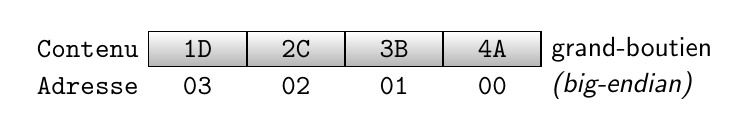
\begin{tikzpicture}[remember picture,%
        every node/.style={font=\ttfamily,anchor=west}, box/.style={text
          width=10mm,text centered,draw=black, top color=white,bottom
          color=black!30},%
        adr/.style={text width=10mm,text centered,
          anchor=north},baseline=(b0.base)]%
        \node (b0) {Contenu}; \node[anchor=north] (ba0) at (b0.south)
        {Adresse}; \node[box] (b1) at (b0.east) {1D}; \node[box] (b2) at
        (b1.east) {2C}; \node[box] (b3) at (b2.east) {3B}; \node[box] (b4) at
        (b3.east) {4A}; \node[adr] (ba1)at (b1.south) {03}; \node[adr] (ba2)at
        (b2.south) {02}; \node[adr] (ba3)at (b3.south) {01}; \node[adr]
        (ba4)at (b4.south) {00}; \node[font=\sffamily] (bef) at (b4.east)
        {grand-boutien}; \node[font=\sffamily\itshape] (bee) at (ba4.east)
        {(big-endian)};
      \end{tikzpicture} %
      \only<4-|handout:0>{\begin{tikzpicture}[remember picture,overlay, every
          path/.style={stealth-,thick,blue,opacity=.5}]%
          \foreach \i/\j/\z in {1/4/2,2/3/1.7,3/2/1.3,4/1/1} { \draw
            (b\j.north)--++(0,\z ex)-|($(d\i.south)+(0,-1ex)$) --(d\i.south);
          }
        \end{tikzpicture}
      }
    \end{itemize}
  \item<3-> little-endian: 6502, x86, VAX.
  \item<4-> big-endian: Motorola 68000, SPARC, System/370.
  \item<5-> bi-endian: ARM, PowerPC (sauf G5), MIPS.
  \item<5-> Les bi-boutiens ont un mode par défaut (big-endian pour PowerPC,
    little-endian pour IA-64).
  \end{itemize}
\end{frame}
\begin{exercice}
  \begin{exercicelet}{Stockage d'une date (suite)}
    \begin{questions}
    \item On veut stocker la date du 24 décembre -4 à 21h45 dans un système 32
      bits. Calculez les valeurs à stocker en hexadécimal (hormis l'adresse du
      fuseau horaire). Vous prendrez comme valeur d'adresse pour le fuseau
      horaire 0x12345678.
    \item Écrivez, les uns après les autres, les octets qui composent cette
      date si on est dans un système 32 bits \emph{big-endian}
    \item Écrivez, les uns après les autres, les octets qui composent cette
      date si on est dans un système 32 bits \emph{little-endian}
    \end{questions}
  \end{exercicelet}
\end{exercice}
\subsection{La compression}
\begin{exercice}
  \begin{exercicelet}{Information intrinsèque}
    \begin{questions}
    \item Si vous lancez une pièce de monnaie 20 fois en l'air, est-ce que
      vous avez plus de chance de tomber sur 20 fois face (F), 10 fois
      face-pile (FP), ou sur FPFPPFFFPPPPFPFFPPFP?
    \item Quelle est la quantité d'information contenue dans la suite binaire
      110111001001 ?  Et dans la suite binaire 000000000000 ? Et dans la suite
      binaire 010101010101 ?
    \item Est-ce qu'on pourrait écrire certaines de ces suites de façons plus
      courtes ? Proposez-en.
    \end{questions}
  \end{exercicelet}
\end{exercice}
\begin{frame}{La compression de données sans pertes}
  \begin{block}{Complexité de Kolmogorov}
    \begin{itemize}
    \item[\ddialoginformation] La complexité d'une suite binaire est le
      programme le plus court qui permet de l'écrire (dans un langage
      adéquat).
      
    \item[\ddialogwarning] Pour certaines suites, le programme le plus court
      est celui qui les contient. C'est lié à la notion d'aléatoire en
      \emph{calculabilité}.

    \item[\ddialogerror] Cette complexité ne peut pas être calculée par un
      programme. Par contre, il est possible de trouver des programmes plus
      courts pour la plupart des données usuelles. C'est la
      \textbf{compression}!
    \end{itemize}
  \end{block}
  \begin{block}{Compression}
    La compression permet d'économiser de la place sur les disques et en
    mémoire.

    Elle pénalise l'accès direct aux données. Elle se paye par des calculs de
    \emph{décompression} pour y accéder.

    En gagnant de la place sur le disque dur, elle permet d'accélérer le
    traitement des données, la lecture depuis le disque étant beaucoup plus
    lente que les calculs pour décompresser en général.
  \end{block}
\end{frame}
\begin{frame}{Les utilitaires classiques}
  \begin{block}{L'archivage}
    \begin{itemize}
    \item[\dialogwarning] L'archivage consiste à transformer toute une
      hiérarchie de fichiers en un fichier unique.
    \item[\dialogerror] Ce n'est pas de la compression.
    \item Souvent couplé à une ou plusieurs méthodes de compression.
    \item Utilitaire \texttt{tar} sous Unix, programmes commerciaux
      \texttt{zip} ou \texttt{rar}.
    \end{itemize}
  \end{block}
  \begin{block}{Les formats classiques}
    \begin{itemize}
    \item \texttt{gzip} utilise le codage de Lempel-Ziv (extension usuelle:
      \texttt{gz})
    \item \texttt{zip} utilise le codage de Lempel-Ziv et de Huffman par
      dessus (extension usuelle: \texttt{zip}, mais aussi d'autres formats:
      \texttt{jar}, \texttt{odt})
    \item \texttt{rar} (logiciel commercial) utilise le codage de Lempel-Ziv
      avec des techniques de prédiction PPM par dessus (extension usuelle:
      \texttt{rar})
    \end{itemize}
  \end{block}
\end{frame}
\begin{frame}{La compression RLE}{Codage par plages}
  La compression RLE (pour \emph{Run Length Encoding}) est une des
  compressions les plus simples: on transforme une suite de symboles en une
  suite de paires (nombre de symboles à répéter -- symbole). Par exemple
  00000011110011 se code \textbf{6}0\textbf{4}1\textbf{2}0\textbf{2}1.

  Il peut mener à une chaîne plus grande que l'originale (par exemple pour
  010101: \textbf{1}0\textbf{1}1\textbf{1}0\textbf{1}1\textbf{1}0\textbf{1}1).

  Le compte est souvent codé sur une taille fixe (un octet). Lorsqu'on
  dépasse, on peut découper en plusieurs \emph{runs} de longueur maximale
  (sauf le dernier). Exemple: \textbf{255}0\textbf{45}0 pour un chaîne de 300
  fois {0}.

  Lorsqu'on a seulement deux symboles, on peut ne noter que le compte, pas le
  symbole. On autorise alors les \emph{runs} de 0 caractères, et on indique le
  caractère initial. Exemple: 0\textbf{255} \textbf{0} \textbf{45} \textbf{1}
  pour 300 zéros suivis d'un 1.
\end{frame}
\begin{exercice}
  \begin{exercicelet}{Compression RLE}
    \begin{questions}
    \item Voilà des suites à compresser avec la compression RLE:
      \begin{itemize}
      \item 00001111001010000111111
      \item 111211211111221312211131122211113213211
      \item 0110100110010110
      \end{itemize}
    \end{questions}
  \end{exercicelet}
  \begin{exercicelet}{Protocole de fax}
    \begin{questionshome}
    \item
      \begin{minipage}[t]{.5\linewidth}
        Un fax est une suite de points noirs et blancs. En utilisant les
        notations du RLE binaire données dans le cours, décrivez l'image à
        droite. On part en haut à gauche de l'image, on part à droite et on
        reprend à la fin de chaque ligne à la ligne suivante à gauche.
      \end{minipage}\hfill
      \begin{minipage}[t]{.2\linewidth}
        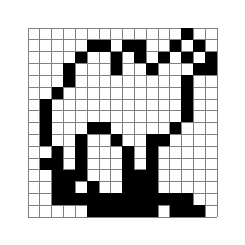
\begin{tikzpicture}[baseline={([yshift={-\ht\strutbox}]current bounding box.north)},scale=.15]
          \draw[gray,very thin] (0,0) grid (16,16);
          \foreach \i in {(5,0),(6,0),(7,0),(8,0),(9,0),(10,0),(12,0),(13,0),(14,0),(2,1),%
            (3,1),(4,1),(5,1),(6,1),(7,1),(8,1),(9,1),(10,1),(11,1),(12,1),(13,1),%
            (2,2),(3,2),(5,2),(8,2),(9,2),(10,2),%
            (2,3),(3,3),(4,3),(8,3),(9,3),(10,3),%
            (1,4),(2,4),(4,4),(8,4),(10,4),%
            (2,5),(4,5),(8,5),(10,5),(1,6),(4,6),(7,6),(10,6),(11,6),%
            (1,7),(5,7),(6,7),(12,7),(1,8),(13,8),(1,9),(13,9),(2,10),(13,10),%
            (3,11),(13,11),(3,12),(7,12),(10,12),(14,12),(15,12),%
            (4,13),(7,13),(9,13),(11,13),(13,13),(15,13),%
            (5,14),(6,14),(8,14),(9,14),(12,14),(14,14),(13,15)} {
            \fill \i rectangle ++(1,1);
          }
        \end{tikzpicture}
      \end{minipage}\hfill\null
    \end{questionshome}
  \end{exercicelet}
\end{exercice}

% Local Variables:
% TeX-master: "archi05"
% TeX-PDF-mode: t
% fill-column: 78
% coding: utf-8-unix
% mode-require-final-newline: t
% mode: latex
% mode: flyspell
% ispell-local-dictionary: "francais"
% End:
